\documentclass[aspectratio=169,11pt]{beamer}

\usepackage{graphicx}
\usepackage{tikz}
\usetikzlibrary{positioning,arrows.meta}
\usepackage{xcolor}
\usepackage{booktabs}
\usepackage{tabularx}
\usepackage{array}
\usepackage{ragged2e}

\definecolor{GEUBlue}{RGB}{20,55,105}
\definecolor{GEULightBlue}{RGB}{238,244,251}
\definecolor{GEUGrey}{RGB}{90,90,90}
\definecolor{GEULightGrey}{RGB}{245,246,248}

\usetheme{default}
\setbeamertemplate{navigation symbols}{}
\setbeamertemplate{blocks}[rounded][shadow=false]
\setbeamercolor{normal text}{fg=black,bg=white}
\setbeamercolor{frametitle}{fg=GEUBlue}
\setbeamercolor{structure}{fg=GEUBlue}
\setbeamercolor{block title}{fg=GEUBlue,bg=GEULightBlue}
\setbeamercolor{block body}{fg=black,bg=GEULightBlue}
\setbeamerfont{frametitle}{size=\Large,series=\bfseries}

% Replace with the actual logo filename
\newcommand{\GEULogo}{pbl format/graphicera_logo.png}

% Header and footer
\setbeamertemplate{headline}{%
  \begin{tikzpicture}[remember picture,overlay]
    \node[anchor=north east,xshift=-0.30cm,yshift=-0.12cm]
      at (current page.north east)
      {\includegraphics[height=0.62cm]{\GEULogo}};
  \end{tikzpicture}
  \vspace{0.72cm}
}
\setbeamertemplate{frametitle}{%
  \vspace{0.03cm}
  \insertframetitle\par
  \vspace{0.04cm}
  \textcolor{GEUBlue}{\rule{\textwidth}{0.9pt}}
  \vspace{0.03cm}
}
\setbeamertemplate{footline}{%
  \leavevmode
  \hbox{%
  \begin{beamercolorbox}[wd=.82\paperwidth,ht=0.32cm,dp=0.10cm,leftskip=.3cm]{author in head/foot}
    \tiny Department of Computer Science \& Engineering | Graphic Era (Deemed to be University)
  \end{beamercolorbox}%
  \begin{beamercolorbox}[wd=.18\paperwidth,ht=0.32cm,dp=0.10cm,rightskip=.3cm]{date in head/foot}
    \hfill\tiny\insertframenumber/\inserttotalframenumber
  \end{beamercolorbox}}
}

\newcommand{\smallnote}[1]{\vspace{0.08cm}{\scriptsize\color{GEUGrey}#1}}
\newcommand{\placeholder}[1]{#1}

\title{\textbf{Project-Based Learning}\\[2mm]\large Phase-I Evaluation}
\author{\textbf{Project Title}\\Team ID: XXXX}
\institute{Department of Computer Science \& Engineering\\Graphic Era (Deemed to be University), Dehradun}
\date{Academic Session 2026--27}

\begin{document}

% 1
\begin{frame}[plain]
\begin{tikzpicture}[remember picture,overlay]
\draw[GEUBlue,line width=3pt] (current page.north west) -- (current page.north east);
\node[anchor=north east,xshift=-0.45cm,yshift=-0.35cm] at (current page.north east)
{\includegraphics[height=1.0cm]{\GEULogo}};
\node[align=center,text width=.84\paperwidth] at ([yshift=.25cm]current page.center)
{{\color{GEUBlue}\fontsize{26}{30}\selectfont\bfseries PROJECT-BASED LEARNING}\\[3mm]
 {\fontsize{18}{22}\selectfont PHASE-I EVALUATION}\\[7mm]
 {\color{GEUGrey}\Large\bfseries Personal Finance / Expense Splitter}\\[3mm]
 {\color{GEUBlue}\normalsize Team ID: DSCPP-III-2026-T272}};
\node[align=center,anchor=south,yshift=.42cm] at (current page.south)
{\bfseries Department of Computer Science \& Engineering\\
Graphic Era (Deemed to be University), Dehradun\\[-1mm]
\scriptsize Academic Session 2026--27};
\end{tikzpicture}
\end{frame}

% 2
\begin{frame}{Team \& Mentor Details}
\begin{columns}[T,totalwidth=\textwidth]
\column{.48\textwidth}
\begin{block}{Team Information}
\begin{tabular}{@{}ll@{}}
\textbf{Team ID:} & DSCPP-III-2026-T272\\
\textbf{Semester:} & 3rd\\
\textbf{Section:} & ML1, ML2, ML3\\
\textbf{Domain:} & FinTech
\end{tabular}
\end{block}
\column{.48\textwidth}
\begin{block}{Team Members}
1.\quad Tanmay Kumar -- 2510370439\\
2.\quad Sparsh Saxena -- 2510370313\\
3.\quad Hemang Sethi -- 2510370341\\
\end{block}
\end{columns}
\vspace{2mm}
\begin{block}{Mentor}
Mr. Yuvraj Joshi
\hfill
\textbf{Interactions completed: 2  } 
\end{block}
\end{frame}

% 3
\begin{frame}{Problem Statement \& Motivation}
\small
\begin{block}{Problem Statement}
Groups struggle to track shared expenses (food, travel, accommodation) and to settle them with the fewest transactions, especially across currencies.
\end{block}
\vspace{2mm}
\begin{columns}[T,totalwidth=\textwidth]
\column{.48\textwidth}
\textbf{\color{GEUBlue}Motivation}
\begin{itemize}\itemsep1pt
\item Manual tracking via notes, spreadsheets, or chats
\item Calculation errors, forgotten payments, disputes
\item Minimizing settlements by hand is slow, worse across currencies
\end{itemize}
\column{.48\textwidth}
\textbf{\color{GEUBlue}Target Users / Stakeholders}
\begin{itemize}\itemsep1pt
\item Primary: friends, roommates, classmates, travel groups
\item Secondary: hostel/mess groups, trip organizers
\item Benefit: clear, automatic, error-free settlement
\end{itemize}
\end{columns}
\end{frame}

% 4
\begin{frame}{Objectives}
\small
\textbf{\color{GEUBlue}Project Objectives}
\vspace{2mm}
\begin{enumerate}\itemsep3pt
\item Develop an OOPs C++ application using User, Group, and Transaction classes.
\item Let users create groups and record shared expenses.
\item Auto-calculate each member's share, paid amount, and balance; use operator overloading for settlement operations.
\item Handle varied group sizes, scenarios, and currencies via templates.
\item Demonstrate transaction-minimizing settlement with future scalability.
\end{enumerate}
\vfill
\begin{center}
\colorbox{GEULightBlue}{\parbox{.80\textwidth}{\centering
\textbf{Key Objective:} Automatically compute each member's balance and generate the minimum number of transactions needed to settle a group's shared expenses.}}
\end{center}
\end{frame}

% 5
\begin{frame}{Proposed Solution}
\footnotesize
\begin{columns}[T,totalwidth=\textwidth]
\column{.48\textwidth}
\textbf{\color{GEUBlue}Proposed Approach}
\begin{enumerate}\itemsep2pt
\item Input: register users/groups, record transactions via console menu
\item Processing: split each expense among selected members
\item Logic: Balance = Paid $-$ Owed, per user
\item Storage: in-memory STL vectors + basic file handling
\item Output: balances and settlement plan on console
\end{enumerate}
\column{.48\textwidth}
\textbf{\color{GEUBlue}Key Features}
\begin{itemize}\itemsep2pt
\item Group/member management (add, search, display)
\item Automatic expense splitting and share calculation
\item Balance tracking: paid vs. owed
\item Debt-settlement that minimizes transactions
\item Multi-currency support via C++ templates
\end{itemize}
\end{columns}
\vfill
\smallnote{Clearly explain how the proposed solution addresses the identified problem.}
\end{frame}

% 6
\begin{frame}{Integration of PBL Course Concepts}
\scriptsize
\begin{center}
\renewcommand{\arraystretch}{1.25}
\begin{tabularx}{.96\textwidth}{@{}>{\bfseries}p{3.0cm}X p{2.5cm}@{}}
\toprule
Course & Concepts Applied & Project Module\\
\midrule
Data Structures in C & Vectors and array-based storage, searching, and sorting used to organize users, groups, and transaction records & User/Group Manager, Data Storage Layer\\
OOPs with C++ & Classes (User, Group, Transaction), encapsulation, constructors, operator overloading, templates, STL & Expense \& Split Engine, Balance \& Settlement Module\\
\bottomrule
\end{tabularx}
\end{center}
\vfill
\begin{center}
\colorbox{GEULightBlue}{\parbox{.86\textwidth}{\centering
\textbf{Requirement:} Demonstrate meaningful integration of both subjects in \textbf{one} project.}}
\end{center}
\end{frame}

% 7
\begin{frame}{System Architecture / Workflow}
\begin{center}
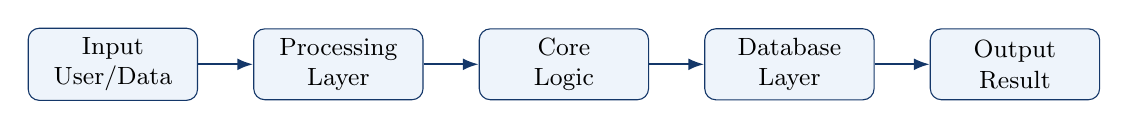
\begin{tikzpicture}[
node distance=7mm,
box/.style={rectangle,rounded corners,draw=GEUBlue,fill=GEULightBlue,
minimum width=2.15cm,minimum height=9mm,align=center,font=\small},
arrow/.style={-{Latex[length=2mm]},thick,draw=GEUBlue}
]
\node[box] (a) {Input\\User/Data};
\node[box,right=of a] (b) {Processing\\Layer};
\node[box,right=of b] (c) {Core\\Logic};
\node[box,right=of c] (d) {Database\\Layer};
\node[box,right=of d] (e) {Output\\Result};
\draw[arrow] (a)--(b); \draw[arrow] (b)--(c); \draw[arrow] (c)--(d); \draw[arrow] (d)--(e);
\end{tikzpicture}
\end{center}
\vspace{3mm}
\begin{columns}[T,totalwidth=\textwidth]
\column{.48\textwidth}
\small
\textbf{\color{GEUBlue}Major Components}
\begin{itemize}\itemsep1pt
\item User / Group Manager -- add, search, manage members
\item Expense \& Split Engine -- records transactions, computes shares
\item Balance \& Settlement -- calculates balances, minimizes transactions
\end{itemize}
\column{.48\textwidth}
\small
\textbf{\color{GEUBlue}Data / Control Flow}
\begin{itemize}\itemsep1pt
\item Console UI passes input to the business logic layer
\item Business logic operates on core classes (User, Group, Transaction)
\item Output: balances and a minimized settlement plan
\end{itemize}
\end{columns}
\end{frame}

% 8
\begin{frame}{Technology Stack \& Methodology}
\begin{columns}[T,totalwidth=\textwidth]
\column{.48\textwidth}
\begin{block}{Technology Stack}
\begin{itemize}\itemsep2pt
\item Programming: C++ (OOP, STL)
\item Database: PostgreSQL (via libpqxx), for persistent multi-user storage
\item Tools / Framework: C++ STL, CMake
\item IDE: Visual Studio Code
\item Version Control: Git / GitHub
\end{itemize}
\end{block}
\column{.48\textwidth}
\begin{block}{Development Methodology}
\begin{enumerate}\itemsep2pt
\item Requirement Analysis
\item System Design
\item Implementation
\item Testing
\item Evaluation
\end{enumerate}
\end{block}
\end{columns}
\vfill
\begin{center}
\smallnote{Justify the selection of technologies and methodology.}
\end{center}
\end{frame}

% 9
\begin{frame}{Initial Progress \& Team Contribution}
\small
\begin{columns}[T,totalwidth=\textwidth]
\column{.44\textwidth}
\textbf{\color{GEUBlue}Progress Achieved}
\begin{itemize}\itemsep2pt
\item Literature study of expense-splitting approaches done
\item Requirements identified: groups, entry, balances, settlement
\item Architecture prepared: User/Group/Transaction classes
\item Initial module: core class skeletons, menu flow
\item Test scenarios identified: hostel, trips, shopping
\end{itemize}
\column{.52\textwidth}
\textbf{\color{GEUBlue}Individual Contribution}
\vspace{2mm}
\scriptsize
\begin{tabularx}{\textwidth}{@{}>{\raggedright\arraybackslash}p{2.1cm}>{\raggedright\arraybackslash}p{1.5cm}>{\raggedright\arraybackslash}X@{}}
\toprule
Member & Role & Contribution\\
\midrule
Tanmay Kumar & Lead & System design and class architecture; team coordination\\
Sparsh Saxena & Developer & Core C++ implementation: expense recording and split logic\\
Hemang Sethi & Docs/ Testing & Test scenarios, documentation, proposal write-up\\
\bottomrule
\end{tabularx}
\end{columns}
\end{frame}

% 10
\begin{frame}{Roadmap, Expected Outcomes \& References}
\footnotesize
\begin{columns}[T,totalwidth=\textwidth]
\column{.47\textwidth}
\textbf{\color{GEUBlue}Roadmap}
\begin{enumerate}\itemsep1pt
\item Phase-I: Proposal \& Design
\item Phase-II: Development
\item Phase-III: Final Implementation
\end{enumerate}
\vspace{1mm}
\textbf{\color{GEUBlue}Expected Outcomes}
\begin{itemize}\itemsep1pt
\item Working console prototype for expense splitting
\item Fewer settlements via debt-minimization algorithm
\item Useful for hostels, trips, shared households
\item Future: web/mobile UI, live rates, DBMS storage
\end{itemize}
\column{.47\textwidth}
\textbf{\color{GEUBlue}References}
\begin{enumerate}\itemsep1pt
\item cppreference.com -- C (en.cppreference.com/w/c)
\item cppreference.com -- C++ book list
\item cppreference.com -- C++ \& STL
\item GEU CSE Dept. (2026) -- DSA C/C++ handout
\end{enumerate}
\vfill
\begin{center}
\colorbox{GEUBlue}{\parbox{.78\textwidth}{\centering\color{white}\textbf{Thank You}\\Questions \& Suggestions}}
\end{center}
\end{columns}
\end{frame}

\end{document}